% Figure s06f01_stoner (Session 6): a graphical reading of the Stoner criterion.
% The image is rendered by figures/blender/s06f01_stoner.py; the coordinates of the labels come from
% figures/blender/out/s06f01_stoner*_anchors.tex. Build with figures/blender/build_figure.sh s06f01_stoner.
\documentclass[11pt,tikz,border=0pt]{standalone}
\usepackage[T1]{fontenc}
\usepackage{amsmath,amssymb,graphicx,bm}
\usepackage{xcolor}
\usetikzlibrary{arrows.meta,calc}
% The three label colors of the figures, with the same values as in src/figures_preamble.tex.
\definecolor{aqmaccent}{RGB}{31,78,121}
\definecolor{aqmbroken}{RGB}{168,42,34}
\definecolor{aqmmuted}{RGB}{125,125,125}

% Shared TikZ styles of the overlays: axis arrows drawn on top of the renders, between anchors
% written by the scripts, so that they can be adjusted without rendering again.
\tikzset{
  axarrow/.style={line width=0.6pt, draw=black!70, -{Stealth[length=4.5pt,width=3.5pt]}},
  axlbl/.style={font=\small, inner sep=1.5pt},
}
% A discrete color key: \aqmkey{(x,y)}{color 1}{label 1}{color 2}{label 2} draws two swatches in a
% column with their labels, anchored at its north west corner. The colors are the sRGB values
% used in the render, defined below.
\definecolor{keypos}{RGB}{118,158,198}
\definecolor{keyneg}{RGB}{214,150,132}
\definecolor{keyup}{RGB}{224,62,40}
\definecolor{keydown}{RGB}{40,92,200}
\definecolor{keydark}{RGB}{31,78,121}
\definecolor{keylight}{RGB}{118,158,198}
\newcommand{\aqmkey}[5]{%
  \begin{scope}[shift={#1}]
    \fill[#2, draw=black!40, line width=0.3pt] (0,-0.32) rectangle (0.32,0);
    \node[font=\small, anchor=west, inner sep=1.5pt] at (0.38,-0.16) {#3};
    \fill[#4, draw=black!40, line width=0.3pt] (0,-0.74) rectangle (0.32,-0.42);
    \node[font=\small, anchor=west, inner sep=1.5pt] at (0.38,-0.58) {#5};
  \end{scope}}
% The same key in one row, for a figure with no room for a column.
\newcommand{\aqmkeyrow}[5]{%
  \begin{scope}[shift={#1}]
    \fill[#2, draw=black!40, line width=0.3pt] (0,-0.32) rectangle (0.32,0);
    \node[font=\small, anchor=west, inner sep=1.5pt] (k1) at (0.38,-0.16) {#3};
    \fill[#4, draw=black!40, line width=0.3pt] ([xshift=0.25cm]k1.east |- 0,-0.32) rectangle ++(0.32,0.32);
    \node[font=\small, anchor=west, inner sep=1.5pt] at ([xshift=0.63cm]k1.east) {#5};
  \end{scope}}

\newlength{\figw}\setlength{\figw}{18.37cm}   % 1.18 of the text width, before the empty margins of the render are cropped

\begin{document}
\begin{tikzpicture}[lbl/.style={font=\small, inner sep=1.5pt}, pnl/.style={font=\small\bfseries, inner sep=1.5pt}]
  \begin{scope}[shift={(0.00cm,0.00cm)}]
    \setlength{\figw}{18.37cm}
    \node[overlay, anchor=south west, inner sep=0pt] at (0,0)
      {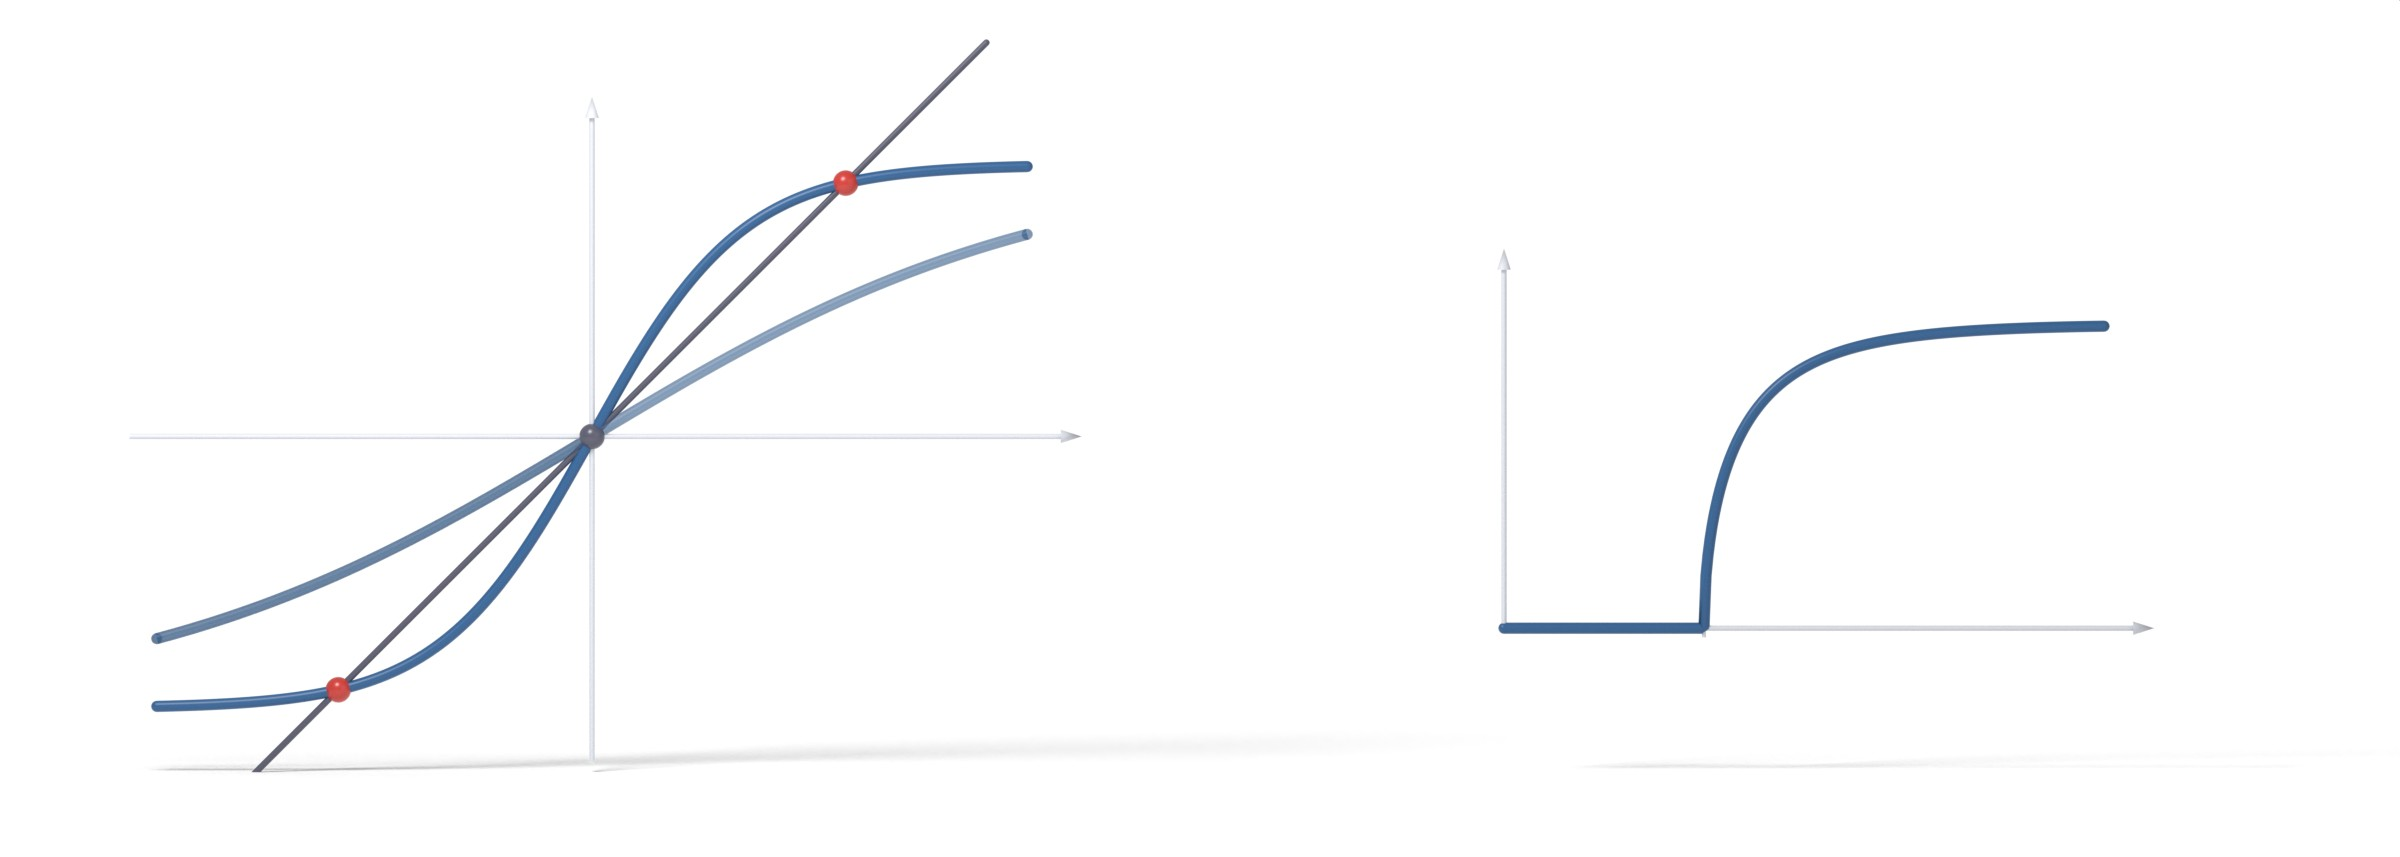
\includegraphics[width=\figw]{../blender/out/s06f01_stoner.jpg}};
    % written by build_figure.sh; the painted part of the image
\path (0.0537\figw,0.0350\figw) rectangle (0.8975\figw,0.3408\figw);

    %% written by figlib.py; x and y in units of the image width
\coordinate (am) at (0.4507\figw,0.1752\figw);
\coordinate (ay) at (0.2467\figw,0.3167\figw);
\coordinate (m0p) at (0.3524\figw,0.2808\figw);
\coordinate (m0m) at (0.1410\figw,0.0696\figw);
\coordinate (sup) at (0.4223\figw,0.2875\figw);
\coordinate (sub) at (0.4223\figw,0.2579\figw);
\coordinate (line) at (0.4076\figw,0.3359\figw);
\coordinate (apanel) at (0.0540\figw,0.3223\figw);
\coordinate (bs) at (0.8975\figw,0.0953\figw);
\coordinate (bm) at (0.6267\figw,0.2534\figw);
\coordinate (bone) at (0.7100\figw,0.0903\figw);
\coordinate (bpanel) at (0.6183\figw,0.2598\figw);

    \node[pnl, anchor=south west] at (apanel) {(a)};
    \node[pnl, anchor=south west] at (bpanel) {(b)};
    \node[lbl, anchor=south east] at (am) {$m$};
    \node[lbl, anchor=west] at (ay) {$y$};
    \node[lbl, anchor=west] at (line) {$y=m$};
    \node[lbl, anchor=west, xshift=3pt, text=aqmaccent] at (sup) {$UD(E_F)>1$};
    \node[lbl, anchor=west, xshift=3pt, text=aqmaccent!60] at (sub) {$UD(E_F)<1$};
    \node[lbl, anchor=south east, text=aqmbroken] at (m0p) {$+m_0$};
    \node[lbl, anchor=north west, text=aqmbroken] at (m0m) {$-m_0$};
    \node[lbl, anchor=south east] at (bs) {$UD(E_F)$};
    \node[lbl, anchor=west] at (bm) {$m_0$};
    \node[lbl, anchor=north] at (bone) {$1$};
  \end{scope}
\end{tikzpicture}
\end{document}
